\documentclass[10pt]{beamer}

\usetheme[progressbar=frametitle]{metropolis}
\usepackage{appendixnumberbeamer}

\usepackage{booktabs}
\usepackage[scale=2]{ccicons}

\usepackage{pgfplots}
\usepgfplotslibrary{dateplot}

\usepackage{xspace}
\newcommand{\themename}{\textbf{\textsc{metropolis}}\xspace}

\title{C Code Generation for SPL in Rust}
\subtitle{Compiler Construction presentation}
\date{}
\author{Oussama Danba}

\begin{document}

\maketitle

\begin{frame}{Table of Contents}
  \setbeamertemplate{section in toc}[sections numbered]
  \tableofcontents[hideallsubsections]
\end{frame}

\section{General Information}
\begin{frame}{Compiler Extension}
    \begin{itemize}
        \item SPL is somewhat limited but is functional. Rather than writing entire programs in SPL it would be desirable to be able to use SPL functions from other languages.
        \begin{itemize}
            \item This requires compilation to machine code for the current architecture.
        \end{itemize}
        \item Rather than doing this myself we can compile to C and then (dynamically) link with the rest.
        \begin{itemize}
            \item Easy interoperability
            \item Cross-platform
            \item Optimized code
        \end{itemize}
    \end{itemize}
\end{frame}

\begin{frame}{General Information}
    \begin{itemize}
        \item Rather than only compiling functions I decided to compile whole programs (globals and main function) since it isn't much more work anyway.
        \item C has no tuples or linked lists so have to do something about that.
        \item Rather than a syntactical translation it is a little more involved.
        \begin{itemize}
            \item Semantic choices made for SPL sometimes conflict with C which requires extra code
        \end{itemize}
        \item C code generator for SPL ended up being around 500 lines of code.
    \end{itemize}
\end{frame}

\section{Implementation Details}
% draw on board why they must be malloced
\begin{frame}{Tuples and Lists}
    \begin{itemize}
        \item Tuples and lists are represented as structs where the members uintptr\_t (pointers without type).
        \begin{itemize}
            \item This allows members to either contain the value or a pointer to another tuple/list.
        \end{itemize}
        \item Tuples and lists are passed by reference so that function calls can modify them. This is done to match the semantics of SPL.
        \begin{itemize}
            \item As a result tuples/lists must be on the heap rather than on the stack. If a function adds an element to the linked list this element must still be guaranteed to be valid later.
        \end{itemize}
    \end{itemize}
\end{frame}

\begin{frame}{Tuples and Lists}
    \begin{itemize}
        \item Whenever tuples and lists are used the generated code inserts the necessary casts. This can be done since all necessary type information is available.
        \item Empty list is again encoded as the tail pointing to 0x0.
    \end{itemize}
    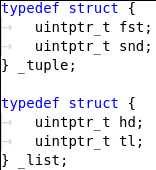
\includegraphics[width=0.4\textwidth]{presentation4/1.png}
\end{frame}

\begin{frame}{Code Generation for Expressions}
    \begin{itemize}
        \item First thing to implement was code generation for expressions.
        \item The literals are easy because they \textit{are} a syntactical translation. Some other expressions require multiple lines of C code.
        \item Creating an empty list for example generates the following:
        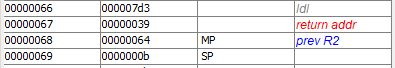
\includegraphics[width=0.9\textwidth]{presentation4/2.png}\\
        Technically a calloc would have sufficed here but for consistency with the rest I use a malloc.
    \end{itemize}
\end{frame}

\begin{frame}{Code Generation for Expressions}
    \begin{itemize}
        \item Other examples or requiring multiple lines of C code are function calls, tuples and identifiers.
        \item A function call can have in-line expressions that have to be evaluated (creating a list that is directly passed for example). Trying to do this in-line is needlessly complex. A C compiler will optimize it out anyway.
        \item Since tuples are malloced they also require multiple lines. Can not use a calloc since fst and snd actually need to be set to a value.
        \item Asking for the head of an identifier can possibly be asking for the head of an empty list. There needs to be run-time checking for this.
    \end{itemize}
\end{frame}

\begin{frame}{Code Generation for Expressions}
    \begin{itemize}
        \item The following example demonstrates why expressions are evaluated on multiple line\\
        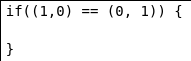
\includegraphics[width=0.5\textwidth]{presentation4/3.png}\\
        This requires two mallocs, setting the elements, and doing equality for the elements. As a result this is translated to evaluating the expression before the if-statement and then passing in a boolean.
    \end{itemize}
\end{frame}

\begin{frame}{Code Generation for Expressions}
    \begin{itemize}
        \item The more interesting (and difficult) expressions are the binary operators.
        \item When making the code generator for SSM I made an explicit choice not to allow short-circuiting of boolean operators.
        \begin{itemize}
            \item \texttt{a \&\& b} will always evaluate a and b. There is no implicit control flow in this regard!
            \item Thus for binary operators the left and right side are always evaluated first.
        \end{itemize}
    \end{itemize}
\end{frame}

\begin{frame}{Code Generation for Expressions}
    \begin{itemize}
        \item Most difficult binary operator to implement was \texttt{==/!=}.
        \begin{itemize}
            \item When generating code for SSM I decided that equality would verify values are the same rather than references.
        \end{itemize}
        \item C equality for structs (thus tuples/lists) works on references instead of members.
        \begin{itemize}
            \item The generated C code must account for this. Including nested tuples/lists.
            \item Tuple equality can be generated by the SPL compiler directly.
            \item Lists can grow dynamically so are generated as a while-loop (with some checking).
        \end{itemize}
    \end{itemize}
\end{frame}

\begin{frame}{Variable Shadowing}
    \begin{itemize}
        \item Variable shadowing works differently in SPL than C (at least, for my semantics). The following is allowed in SPL:
        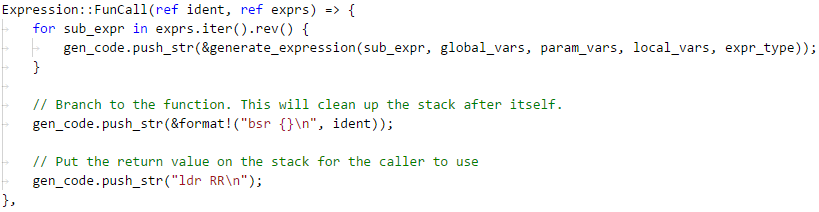
\includegraphics[width=0.4\textwidth]{presentation4/4.png}
        \item This does not work in C. You can't shadow globals/parameters with a local using the same name (and a different type).
        \begin{itemize}
            \item As a result locals have random name in the generated code.
            \item A mapping is established so the compiler always\footnotemark  knows which ``real'' name to use.
        \end{itemize}
    \end{itemize}
    \footnotetext[1]{When making these slides I found a bug where the mapping was not updated.}
\end{frame}

\begin{frame}{Code Generation for Globals}
    \begin{itemize}
        \item Another problem is that C globals must be known at compile-time. The following is allowed in SPL:
        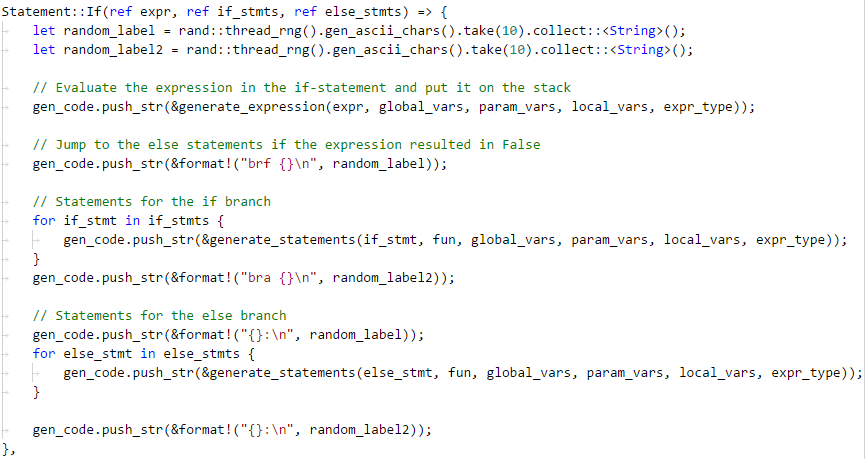
\includegraphics[width=0.4\textwidth]{presentation4/5.png}
        \item The equivalent C code will not compile.
        \begin{itemize}
            \item C requires global initializations to be constant at compile-time.
        \end{itemize}
    \end{itemize}
\end{frame}

\begin{frame}{Code Generation for Globals}
    \begin{itemize}
        \item Solving the mentioned issue means that declaration and initialization will be split up in the code generator.
        \begin{itemize}
            \item The first thing the C code does is initialize the declared globals.
        \end{itemize}
    \end{itemize}
\end{frame}

\begin{frame}{Code Generation for Statements}
    \begin{itemize}
        \item Code generation for statements is rather trivial as every SPL statement has a direct counterpart in C and the semantics are the same.
        \item As mentioned before there is a little bit of work involved in first evaluating the expressions before passing the results on to the statements.
    \end{itemize}
\end{frame}

\begin{frame}{Code Generation for isEmpty}
    \begin{itemize}
        \item I implemented monomorphic type checking but made an exception for the isEmpty function.
        \item Since the semantic analysis ensures that only lists of \textit{some} type are passed isEmpty is trivial.
        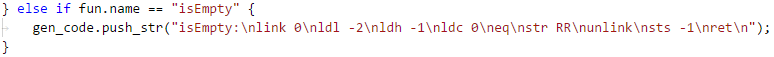
\includegraphics[width=0.6\textwidth]{presentation4/6.png}
    \end{itemize}
\end{frame}

\begin{frame}{Code Generation for print}
    \begin{itemize}
        \item print is overloaded and instead of generating a function for each type print is generated inline.
        \item Like SSM the idea is to implement printing for basic types and use those to implement printing for tuples/lists.
        \begin{itemize}
            \item Basic types are easy as C has printf with format specifiers.
            \item Printing tuples is not very difficult as the type (and thus the amount of nesting) is known at compile-time.
            \item Printing lists is done by rewriting it to a while-loop that continues as long as the list if not empty. In the body the hd of the list is printed.
        \end{itemize}
    \end{itemize}
\end{frame}

\begin{frame}{Example program}
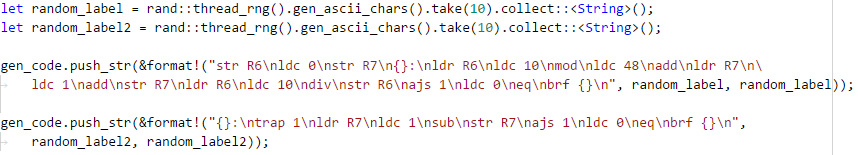
\includegraphics[width=\textwidth]{presentation4/7.png}
\end{frame}

\begin{frame}{Example program C code}
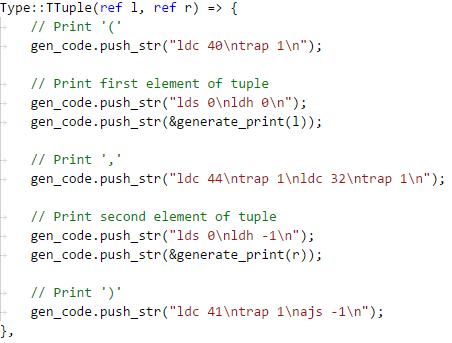
\includegraphics[width=\textwidth]{presentation4/8.png}
\end{frame}

\begin{frame}{Example program output}
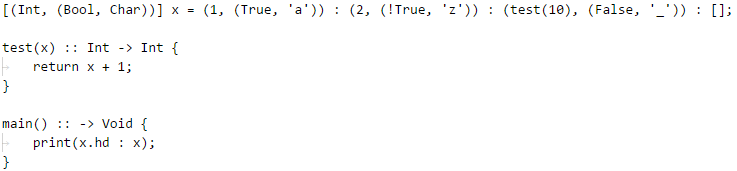
\includegraphics[width=0.2\textwidth]{presentation4/9.png}
\end{frame}

\begin{frame}{Linking}
    \begin{itemize}
        \item As shown the code generation for C works.
        \begin{itemize}
            \item To be able to call these functions from other code simply following the language instructions.
            \item Typically this involved compiling to an object file and then statically linking.
        \end{itemize}
    \end{itemize}
\end{frame}

% Would I do it in Rust again? Absolutely.
% actually more work than expected since you have to emulate semantics
\section{Ending}
\begin{frame}{Afterthoughts}
    \begin{itemize}
        \item More work than expected due to having to emulate the semantics of SPL inside of C.
        \item However, SSM and C code generators have the same semantics!
        \item SPL compiled to C can be linked to other programs and work.
        \item I'm happy with how the compiler turned out
        \begin{itemize}
            \item Would I do it again in Rust? Absolutely.
        \end{itemize}
    \end{itemize}
\end{frame}

{\setbeamercolor{palette primary}{fg=black, bg=yellow}
\begin{frame}[standout]
  Questions?
\end{frame}
}

\begin{frame}{License information}

  Get the source of this theme from

  \begin{center}\url{github.com/matze/mtheme}\end{center}

  The theme \emph{itself} is licensed under a
  \href{http://creativecommons.org/licenses/by-sa/4.0/}{Creative Commons
  Attribution-ShareAlike 4.0 International License}.

  \begin{center}\ccbysa\end{center}

\end{frame}

\end{document}
